% =============================================================================
% reactor-schematic.tex — Simplified pyrolysis/gasification reactor schematic:
% feedstock + heat in, biochar out the bottom, vapor to a condenser splitting
% into bio-oil (condensed) and syngas (non-condensable).
%
% Compiles standalone via: xelatex reactor-schematic.tex
% =============================================================================

\documentclass[border=4pt]{standalone}
\usepackage{tikz}
\usetikzlibrary{arrows.meta, positioning, shapes.geometric}

\definecolor{reactor-fill}{HTML}{E8EDF5}
\definecolor{reactor-border}{HTML}{012169}
\definecolor{aux-fill}{HTML}{FFF7E0}
\definecolor{aux-border}{HTML}{B9975B}
\definecolor{flow-color}{HTML}{1A1A1A}

\tikzset{
  reactor-node/.style={
    draw=reactor-border, fill=reactor-fill, rounded corners=2pt,
    minimum width=2.6cm, minimum height=2.6cm, align=center, font=\small
  },
  aux-node/.style={
    draw=aux-border, fill=aux-fill, rounded corners=2pt,
    minimum width=2.2cm, minimum height=1.0cm, align=center, font=\small
  },
  flow/.style={-{Latex[length=2.5mm]}, thick, draw=flow-color}
}

% -----------------------------------------------------------------------------
% Diagram: Feedstock + heat -> Reactor -> {Biochar (down), Vapor (up) ->
% Condenser -> {Bio-oil, Syngas}}.
% Coordinates (center of each node):
%   reactor    at (0,    0)
%   feedstock  at (-3.2, 0.8)   -- inlet, left of reactor
%   heat       at (-3.2, -0.8)  -- inlet, left of reactor
%   biochar    at (0,   -2.6)   -- outlet, below reactor
%   condenser  at (3.4,  1.5)   -- above-right of reactor
%   biooil     at (6.2,  2.3)
%   syngas     at (6.2,  0.7)
% -----------------------------------------------------------------------------

\begin{document}
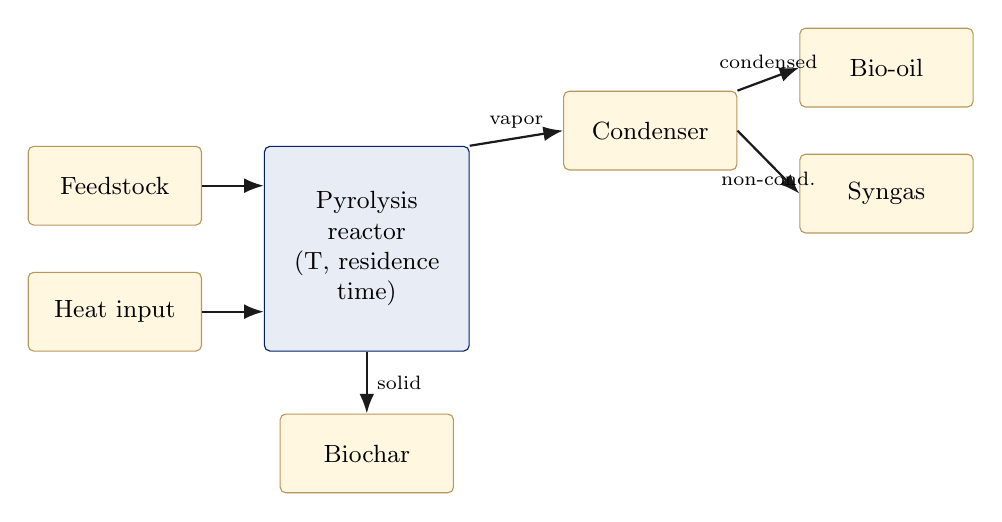
\begin{tikzpicture}
  \node[reactor-node] (reactor)   at (0, 0)      {Pyrolysis\\reactor\\(T, residence\\time)};
  \node[aux-node]      (feedstock) at (-3.2, 0.8)  {Feedstock};
  \node[aux-node]      (heat)      at (-3.2, -0.8) {Heat input};
  \node[aux-node]      (biochar)   at (0, -2.6)    {Biochar};
  \node[aux-node]      (condenser) at (3.6, 1.5)   {Condenser};
  \node[aux-node]      (biooil)    at (6.6, 2.3)   {Bio-oil};
  \node[aux-node]      (syngas)    at (6.6, 0.7)   {Syngas};

  \draw[flow] (feedstock) -- (reactor.west |- feedstock);
  \draw[flow] (heat) -- (reactor.west |- heat);
  \draw[flow] (reactor.south) -- node[midway, right, font=\scriptsize] {solid} (biochar.north);
  \draw[flow] (reactor.north east) -- node[midway, above, font=\scriptsize] {vapor} (condenser.west);
  \draw[flow] (condenser.north east) -- node[midway, above, font=\scriptsize] {condensed} (biooil.west);
  \draw[flow] (condenser.east) -- node[midway, below, font=\scriptsize] {non-cond.} (syngas.west);
\end{tikzpicture}
\end{document}
